\documentclass[twoside]{article}
\usepackage[utf8]{inputenc}
\usepackage{amsmath,amsfonts,amssymb,amsthm,latexsym}
\usepackage[spanish,es-noshorthands]{babel}
\usepackage[T1]{fontenc}
\usepackage{lmodern}
\usepackage{graphicx,hyperref}
\usepackage{tikz,pgf}
\usepackage{marvosym}
\usepackage{multicol}
\usepackage{fancyhdr}
\usepackage[papersize={5.5in,8.5in},left=.75cm,right=.75cm,top=1.5cm,bottom=1.25cm]{geometry}
\usepackage{fancyhdr}
\pagestyle{fancy}
\fancyhead[LE]{\Email iedabgerman@autistici.org}
\fancyhead[RE]{}
\fancyhead[RO]{\url{https://www.autistici.org/mathgerman}}
\fancyhead[LO]{}

\author{Germ\'an Avenda\~no Ram\'irez~\thanks{Lic. Mat. U.D., M.Sc. U.N.}}
\title{\begin{minipage}{.2\textwidth}

\includegraphics[height=1.75cm]{Images/logo-colegio.png}\end{minipage}
\begin{minipage}{.55\textwidth}
\begin{center}
Recomendaciones período 1\\
Aritmética $6^{\circ}$
\end{center}
\end{minipage}\hfill
\begin{minipage}{.2\textwidth}
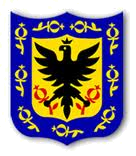
\includegraphics[height=1.75cm]{Images/logo-sed.png} 
\end{minipage}}
\date{}
\thispagestyle{plain}
\begin{document}
\maketitle
\begin{minipage}{.95\textwidth}
\fbox{\textit{No raye ni dañe esta hoja para que pueda usarla otro compañero}}
\end{minipage}
\section*{Taller}
Cada ejercicio o problema debe ser resuelto mostrando los procedimientos o razonamientos para llegar a la respuesta. Éste taller deber resolverse en hoja examen.
\begin{enumerate}
\item Resuelva el siguiente crucinúmero. Realice los procedimientos de cada una de los ejercicios o problemas:
\paragraph*{Horizontales}
\begin{enumerate}
\begin{multicols}{2}
\item[1] $38+45=$
\item[3] $72\div 9=$
\item[4] $23\times 18=$
\item[7] $480\div 12=$
\item[8] $7\times \underline{\hspace*{12pt}}=84$
\item[10] $2\times 2\times 2\times 2\times 3=$
\item[11] $526\times 10=$
\item[13] $93\times 50=$
\item[15] $675+428+325=$
\item[17] $726+483+198=$
\item[20] $2\times 2\times 2\times 2\times 2=$
\item[22] $1008\div 36=$
\item[23] $13\times 3=$
\item[25] $4092\div 6=$
\item[26] $3\times 23=$
\end{multicols}
\end{enumerate}
\paragraph*{Verticales}
\begin{enumerate}
\begin{multicols}{2}
\item[1] $112-28=$
\item[2] $48+135+72+50=$
\item[3] $24\times 34=$
\item[5] $10+4=$
\item[6] $242\times 20=$
\item[9] $715-511=$
\item[12] $112+80+17+13=$
\item[14] $5\times 8\times 16=$
\item[15] $700+336=$
\item[16] $1088-276=$
\item[18] $8\times 6\times 10=$
\item[19] $23\times 32=$
\item[21] $7+7+7+7=$
\item[24] El número mayor de dos dígitos
\end{multicols}
\end{enumerate}
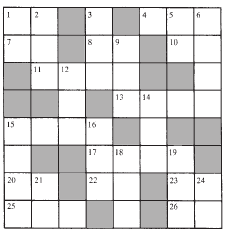
\includegraphics[scale=.9]{Images/crucinumero.png} 
\item Dibuje una línea recta para cada item siguiente:
\begin{enumerate}
\item Muestre que $3+5=5+3$
\item Muestre que $(4\times 2)\times 3=4\times (2\times 3)$
\item Ubique en la recta numérica los número primos entre 25 y 38
\item Ubique en la recta los números compuestos que hay entre 15 y 25
\end{enumerate}
\item Determine el valor numérico de 7 acuerdo a su valor posicional en los siguiente números
\begin{enumerate}
\begin{multicols}{2}
 \item 297
 \item 370
 \item 10\,742
 \item 7\,243
\end{multicols}
\end{enumerate}
 \item Aproxime los siguientes números al lugar indicado
\begin{enumerate}
\item 8296 a las centenas
\item 7406 a las decenas
\item 9516 a las unidades de mil
\end{enumerate} 
\item Aproxime las siguientes operaciones y luego verifíquelas usando el algoritmo usual aprendido.
\begin{enumerate}
\begin{multicols}{2}
\item $79+213=$
\item $923-872=$
\item $983\times 189=$
\item $2098\div 1049=$
\end{multicols}
\end{enumerate}
\item Encuentre:
\begin{enumerate}
\begin{multicols}{2}
\item $3+4\cdot 5=$
\item $(3+4)\cdot 5=$
\item $18\div 3 + 6=$
\item $18\div (3+6)=$
\item $5+2(3+4\times 6)=$
\item $8\div 2+6\times 3=$
\item $[8\div (2+6)]\cdot 3-1=$
\end{multicols}
\end{enumerate}
\item Coloque en los cuadrados dígitos para completar correctamente la adición propuesta:
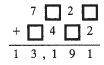
\includegraphics[scale=.75]{Images/adicion.png} 
\item El uso de acero en los Estados Unidos fue de 98'906,000 toneladas métricas en 1990 y de 66'982,686 toneladas métricas en 1940. Encuentre el incremento del uso de acero en USA.
\item Australia producía 6'751,647 onzas de oro en 1990. Si el oro se vendía a \$350 dólares por onza, cual fue el valor total del oro producido por Australia en billones de dólares?
\item Un dólar americano vale aproximadamente \$3,400 pesos colombianos. ¿Cuántos dolares se necesitan para cambiar \$45,000 pesos colombianos?
\end{enumerate}
\section*{Problemas finales}
Soluciones los siguientes problemas
\begin{enumerate}
\item ¿Cuál es el valor del dígito 2 en 320'465,894?
\item ¿Escriba en palabras el número $3'056,070$
\item Un número tiene un 3 en las centenas y centenas de mil, un 7 en las decenas de mil y en las unidades, un 6 en las unidades de mil y un 0 en cualquier otro lugar. ¿Cuál es el número?
\item Identifique los número primos entre 100 y 120
\item Aproxime el producto $45\times 789$ a un dígito que nos sea cero seguido ceros apropiados.
\item Aproxime 49,883 a las unidades de mil
\item Multiplique los dos números 17 y 23. ¿Su producto es un número primo?. Explique
\item Adicione 345 millones a 4'687,349
\item ¿Cuál es la diferencia entre \$5 millones y \$350,000?
\item Brita gasta \$21 dólares para un pin en México. Si el cambio de moneda es de \$1 a 10 nuevos pesos mexicanos, ¿cuántos pesos gastó ella?
\end{enumerate}
\end{document}
